
\chapter{Anhänge}

Für Anhänge gilt, dass das Dokument auch verständlich sein, soll,
wenn Anhänge fehlen würden. Lange Tabellen mit Messdaten können beispielsweise
in den Anhang aufgenommen werden, oder umfangreiche Konstruktionszeichnungen.
Als Beispiel sind hier in Anhang \ref{chap:Wichtige-Abbildung} und
Anhang \ref{chap:Wichtige-Tabelle} Anhänge beigefügt.

\chapter{Aufzählungen und Nummerierungen}

Insbesondere in den Naturwissenschaften ist es häufig sinnvoll statt
einem langen Fließtext eine Aufzählung oder eine Nummerierung zu verwenden.
Aufzählungen dienen:
\begin{itemize}
\item der Übersichtlichkeit
\item der Strukturierung
\item zur Nennung verschiedener Punkte, wenn keine Reihenfolge festgelegt
werden kann.
\end{itemize}
Eine Nummerierung wird verwendet, wenn eine Reihenfolge genannt werden
kann. Als Beispiel seien hier die fünf Sicherheitsregeln der Elektrotechnik
genannt:
\begin{enumerate}
\item Freischalten
\item Gegen Wiedereinschalten sichern
\item Spannungsfreiheit feststellen
\item Erden und Kurzschließen
\item Benachbarte unter Spannung stehende Teile abdecken oder abschranken.
\end{enumerate}

\chapter{Hyperlinks}

Hyperlinks können mit einem Rahmen umfasst werden, der am Display
angezeigt, aber nicht ausgedruckt wird. Dies zeigt die Abbildung \ref{fig:linkmitrahmen}.
Dies ist der Standardfall. Nicht alle PDF-Betrachtungsprogramme heben
hyperlinks optisch hervor. Das Programm SumatraPDF tut dies beispielsweise
nicht.

\begin{figure}
\hfill{}
\includegraphics[width=5cm]{figures/05_rahmenumlinks/mitrahmen}\hfill{}\null

\caption{Hyperlink mit optischer Hervorhebung mit einem blauen Rahmen}
\label{fig:linkmitrahmen}
\end{figure}

Dies kann unterbunden werden mit folgenden Optionen des Paketes hyperref:

\bgroup\inputencoding{latin9}
\begin{lstlisting}
\usepackage[colorlinks=false,pdfborder={0 0 0}]  {hyperref}
\end{lstlisting}
\leavevmode\egroup

Die Abbildung \ref{fig:linkohnerahmen} zeigt das Ergebnis.

\begin{figure}
\hfill{}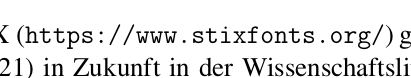
\includegraphics[width=5cm]{figures/05_rahmenumlinks/ohnerahmen}\hfill{}\null

\caption{Hyperlink ohe optischer Hervorhebung mit einem blauen Rahmen}
\label{fig:linkohnerahmen}
\end{figure}


\chapter{Quellcode}

In LaTeX gibt es das Paket Listings, mit dem recht komfortabel Quellcode
in das Dokument aufgenommen werden kann. Hier ist ein Beispiel: 

\lstinputlisting[caption={{Kurzer Batch-Code}},label={kurzerbatchcode}]{figures/02programmlisting/SplitPDFInSinglePages.ps}

Im folgenden Beispiel ist der Code farblich gekennzeichnet.

\lstinputlisting[language=Matlab,caption={Testunterschrift},label={foo}]{figures/04MatlabCode/matlabcode.m}

Hier ist ein weiteres Beispiel, welches einen Seitenumbruch, Listing-Unterschrift
und einen Querverweis (Es handelt sich um das Listing \ref{lstsehrlangeslisting})
auf das Listing enthält:

\lstinputlisting[captionpos=b,label={lstsehrlangeslisting},caption={Unterschrift des sehr langen Quellcodes}]{figures/02programmlisting/SehrLangerQuellCode.txt}

Hier ist ein Listing in einer Zeile \lstinline[language=C]|for(int i = 0, i<5,i++){i--;}print('a');struct A;// Kommentar|

Das ist ein inline-Code ohne Farben:  \lstinline[]|for(int i = 0, i<5,i++){i--;}print('a');struct A;// Kommentar|

\chapter{Zusammenfassung}

Hier wird beschrieben, welche Erkenntnisse sich aus der Arbeit ergeben.
Weiterhin kann hier auch angegeben werden, welche Themen weiter untersucht
werden können oder sollten.
